\documentclass[a4paper]{report}
\usepackage[T1]{fontenc} % Fontes T1
\usepackage[utf8]{inputenc} % Input UTF8
\usepackage[backend=biber, style=ieee]{biblatex} % para usar bibliografia
\usepackage{csquotes}
\usepackage[portuguese]{babel} %Usar língua portuguesa
\usepackage{blindtext} % Gerar texto automaticamente
\usepackage[printonlyused]{acronym}
\usepackage{hyperref} % para autoref
\usepackage{graphicx}
\usepackage{float}
\usepackage{amsmath, amsfonts, amssymb}
\usepackage{caption}

\bibliography{bibliografia.bib}


\begin{document}
%%
% Definições
%
\def\titulo{Cliente para acesso a sonda}
\def\data{20 de Abril de 2018}
\def\autores{Ricardo Ermida, Rodrigo Santos}
\def\autorescontactos{(89187) ricardoermida@ua.pt, (89180) rodrigo.l.silva.santos@ua.pt}
\def\versao{1.0}
\def\departamento{DETI - Universidade de Aveiro}
\def\empresa{Universidade de Aveiro}
\def\logotipo{ua.pdf}
%
%%%%%% CAPA %%%%%%
%
\begin{titlepage}

\begin{center}
%
\vspace*{50mm}
%
{\Huge \titulo}\\ 
%
\vspace{10mm}
%
{\Large \empresa}\\
%
\vspace{10mm}
%
{\LARGE \autores}\\ 
%
\vspace{30mm}
%
\begin{figure}[h]
\center
\includegraphics{\logotipo}
\end{figure}
%
\vspace{30mm}
\end{center}
%
\begin{flushright}
\versao
\end{flushright}
\end{titlepage}

%%  Página de Título %%
\title{%
{\Huge\textbf{\titulo}}\\
{\Large \departamento\\ \empresa}
}
%
\author{%
    \autores \\
    \autorescontactos
}
%
\date{\data}
%
\maketitle

\pagenumbering{roman}

%%%%%% RESUMO %%%%%%
\begin{abstract}
O primeiro passo para o funcionamento da aplicação é a criação de um socket, através do qual é efetuada a conexão ao servidor \textbf{\texttt{xcoa.av.it.pt}}, de seguida é necessário enviar o comando \textbf{\texttt{CONNECT}} para o servidor de modo a receber o\texttt{Token} necessário para a comunicação com o servidor. Para iniciar a recolha dos dados de temperatura, vento e humidade, enviamos o comando \textbf{\texttt{READ}} seguido do token recebido anteriormente. Optámos por aguardar por 2 objetos com a informação de temperatura, vento e humidade, e á medida que eles são recebidos, são guardados num ficheiro \ac{csv}, por fim é feita a média dos valores da temperatura e é mostrado na linha de comandos um conselho sobre o tipo de roupa a levar consoante a temperatura.

\end{abstract}


\tableofcontents
% \listoftables     % descomentar se necessário
% \listoffigures    % descomentar se necessário


%%%%%%%%%%%%%%%%%%%%%%%%%%%%%%%
\clearpage
\pagenumbering{arabic}

%%%%%%%%%%%%%%%%%%%%%%%%%%%%%%%%
\chapter{Introdução}
\label{chap.introducao}

O tema deste relatório será o código desenvolvido para o acesso remoto a uma sonda, de modo a obter dados sobre a temperatura, vento e humidade.

Será feito uma descrição e discução acerca dos aspectos mais importantes do funcionamento da aplicação, com recurso a imagens da execução da aplicação e de alguns testes a algumas partes do código.

Este relatório está dividido em 3 capítulos.

Depois desta introdução, no \autoref{chap.descricao} é feita a descrição do funcionamento da aplicação, este capítulo encontra-se dividido em 3 subcapítulos no primeiro é descrita como é feita a ligação á sonda, no segundo como são recebidos e guardados os objetos \ac{json}, no terceiro subcapítulo apresentamos a nossa opção para o conselho é calculado. Por fim, no \autoref{chap.conclusao} são apresentadas as conclusões retiradas após terminado o trabalho.

\chapter{Descrição e Testes}
\label{chap.descricao}

Para que a aplicação funcionasse corretamente é necessário que o código desenvolvido esteja bem escrito, para sabermos se está ou não bem escrito é preciso realizar testes em diferentes partes do código.

\section{ligação á Sonda}

Quando executamos o programa criamos um socket através do qual entramos no server do xcoa. De seguida criamos uma variavel com o comando "CONNECT" codificamo-la e enviamos o comando para efetuar a ligação ao servidor. Nesta fase fizemos um teste de forma a garantir que a informação que queriamos enviar estava correta e consequentemente que o programa estava a funcionar corretamente, este teste não foi incluído no código final do trabalho.

A imagem a seguir, mostra o resultado desse teste, ou seja, o comando \textbf{\texttt{CONNECT}} codificado que é enviado para o servidor:

\begin{center}
\begin{figure}[H]
\center
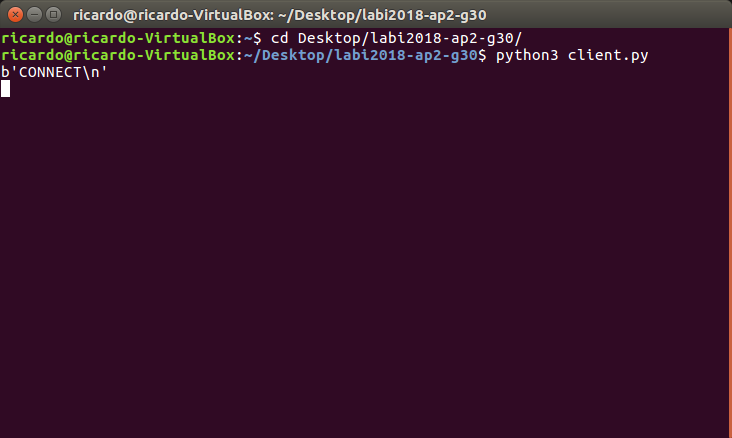
\includegraphics[width=11 cm]{prints/connect.png}
\caption{Teste do comando \textbf{\texttt{CONNECT}}}
\end{figure}
\end{center} 

\section{Receção dos Objetos JSON}

A comunicação entre a sonda e o cliente é feita atravéz de comandos enviados pelo cliente e objetos do tipo \ac{json} enviados pela sonda. Logo é necessário receber esses objetos e ler o seu conteúdo. 

Depois da conexão á sonda estar feita é feita a recolha do objeto \ac{json} com o token, nesta fase é testado se este objeto é recebido corretamente,

\begin{center}
\begin{figure}[H]
\center
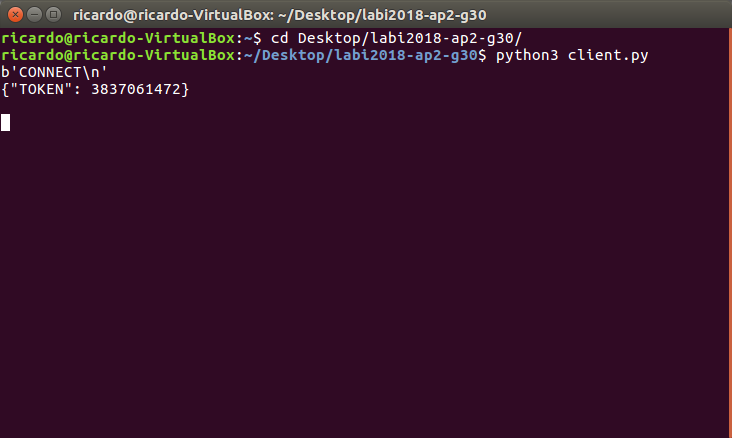
\includegraphics[width=11 cm]{prints/token.png}
\caption{Teste do token}
\end{figure}
\end{center}

abrimos o objeto e criamos o próximo comando a enviar, comando \textbf{\texttt{READ}} seguido do token, o comando é codificado e enviado para o servidor, tal como no comando \textbf{\texttt{CONNECT}} foi testada tambem a codificação do comando \textbf{\texttt{READ}}, 

\begin{center}
\begin{figure}[H]
\center
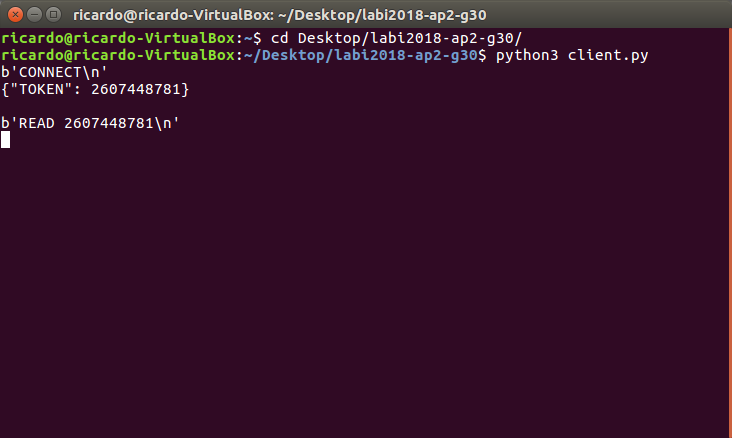
\includegraphics[width=11 cm]{prints/read.png}
\caption{Teste do comando \textbf{\texttt{READ}}}
\end{figure}
\end{center}

de seguida é recolhido e impresso no terminal o objeto de \textbf{\texttt{OK}} enviado pelo servidor. Após a receção do \textbf{\texttt{OK}} é recolhido o primeiro objeto com valores de vento, temperatura e humidade.

\begin{center}
\begin{figure}[H]
\center
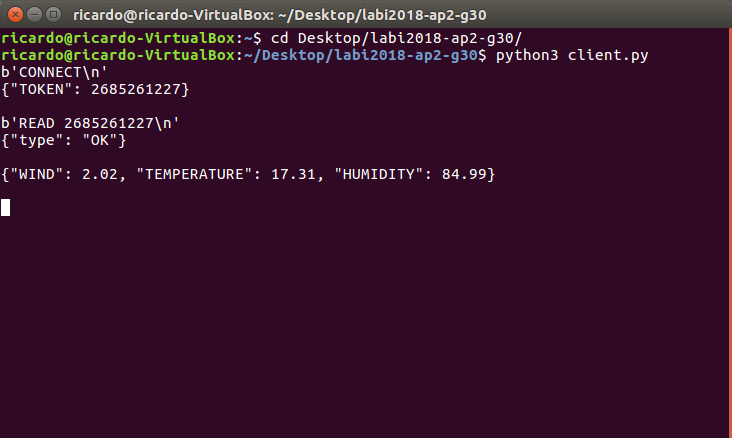
\includegraphics[width=11 cm]{prints/primeiro_valor.png}
\caption{Teste da receção do primeiro objeto do tipo \ac{json}}
\end{figure}
\end{center}

Esses valores são guardados em variáveis, para depois serem armazenados num ficheiro \ac{csv} criado anteriormente, o mesmo acontece com o segundo objeto de valores.

\begin{center}
\begin{figure}[H]
\center
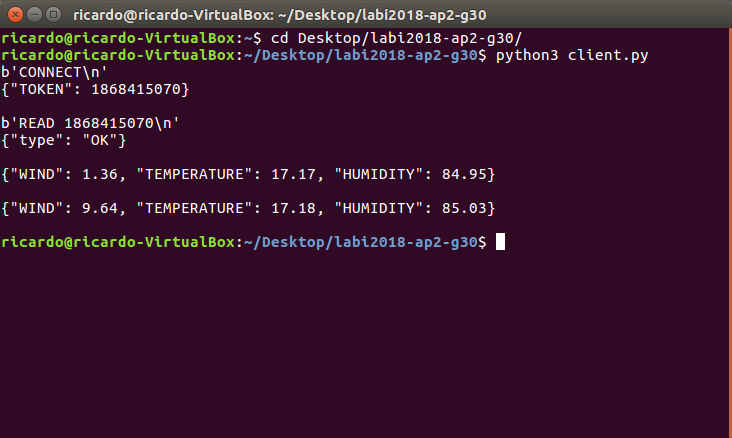
\includegraphics[width=11 cm]{prints/valores_obtidos.png}
\caption{Teste da receção do segundo objeto do tipo \ac{json}}
\end{figure}
\end{center}

\section{Resultados e Conselho}

Nesta parte do trabalho fizemos a média das somas das temperaturas, de modo a conseguir informar o utilizador se estava calor, frio, ou temperatura amena, e o tipo de roupa que deve levar.

\begin{center}
\begin{figure}[H]
\center
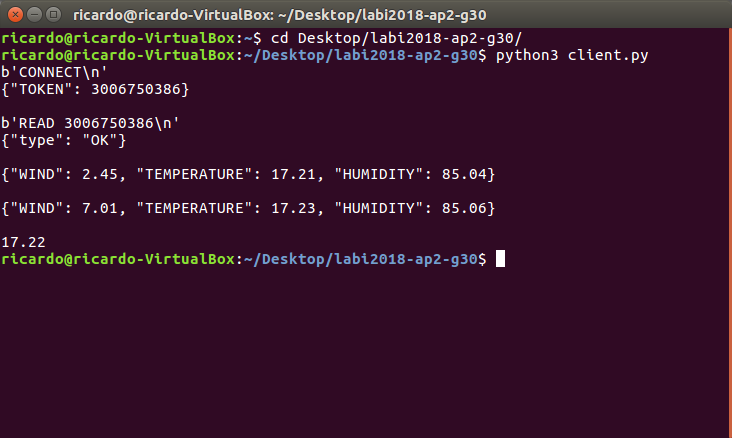
\includegraphics[width=11 cm]{prints/temp.png}
\caption{Teste do cálculo da media das temperaturas}
\end{figure}
\end{center}

Se a temperatura estiver abaixo dos 12 graus o utilizador recebe uma mensagem a dizer que está frio e que deve levar roupa quente, se a temperatura estiver a cima dos 12 graus e abaixo dos 20 graus o utilizador recebe uma mensagem a dizer que a temperatura está agradável e que deve levar roupa amena, se a temperatura estiver a cima dos 20 graus o utilizador recebe uma mensagem a dizer que está calor e que deve levar roupas mais leves.

\chapter{Conclusões}
\label{chap.conclusao}

Após todos os testes unitários executados anteriormente verificamos que o programa funciona corretamente, e tem o aspeto seguinte:

\begin{center}
\begin{figure}[H]
\center
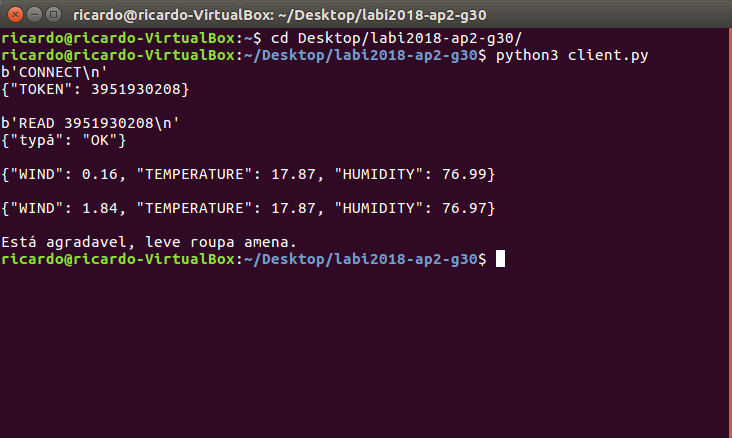
\includegraphics[width=11 cm]{prints/complete.png}
\caption{Programa executado com os testes}
\end{figure}
\end{center}

Para o código final do programa retiramos os testes feitos ao longo deste por questões de simplificação estética.

Com a realização deste projeto aprofundamos as nossas competências em programação na linguagem Pyhton, aplicando esses conhecimentos numa situação real. Este trabalho de aprofundamento foi uma boa maneira para nos preparar para futuros projetos que possamos vir a estar envolvidos que envolvem Python e comunicação com servidores.

\chapter*{Contribuições dos autores}

No desenvolvimento deste trabalho de aprofundamento, ambos os membros do grupo demonstraram o empenho necessário para a sua conclusão.
O Ricardo Ermida executou os testes aos diferentes blocos de código, tendo o Rodrigo Santos desenvolvido o código necessário para a aplicação. O relatório foi feito em conjunto por ambos os membros do grupo. Ambos releram o relatório várias vezes para certificar de que não havia erros de qualquer espécie e para que fosse modificado, se necessário, algum do conteúdo.
Assim o trabalho desenvolvido pelo Rodrigo Santos e pelo Ricardo Ermida foi de 50\% cada um.


%%%%%%%%%%%%%%%%%%%%%%%%%%%%%%%%%
\chapter*{Acrónimos}
\begin{acronym}
\acro{ua}[UA]{Universidade de Aveiro}
\acro{csv}[CSV]{Comma-Separated Values}
\acro{json}[JSON]{JavaScript Object Notation}
\end{acronym}

%%%%%%%%%%%%%%%%%%%%%%%%%%%%%%%%%
\end{document}